\section{Případy užití}
Tato podkapitola se věnuje jednotlivým případům užití, které představují detailnější specifikaci funkčních požadavků. Případy užití poté mohou posloužit jako základ pro~tvorbu uživatelské dokumentace a~také mohou být podkladem pro~tvorbu akceptačních testů. \cite{usecases}

\subsection{Aktéři}
Aktérem (účastníkem) nazýváme uživatele, který bude pracovat se systémem. Celkem uvažujeme čtyři různé aktéry~–~přihlášeného a~nepřihlášeného uživatele, administrátora a~trenéra. Vztahy mezi těmito aktéry jsou popsány v~následujícím textu a~jsou znázorněny na~obrázku \ref{figure:actors}.
\begin{description}
	\item[Nepřihlášený uživatel]\hfill\newline
	Nepřihlášený uživatel má přistup pouze k~přihlášení a~registraci. Po~provedení jedné z~těchto akcí se stane přihlášeným uživatelem.
	\item[Přihlášený uživatel]\hfill\newline
	Přihlášený uživatel má práva, která byla již dříve popsána v~sekci \ref{section:role} u~role registrovaný uživatel. Jelikož je uživatel již přihlášený do~systému, tak nemá přístup k~přihlašovací stránce a~k~registraci.
	\item[Trenér]\hfill\newline
	Práva trenéra vycházejí z~práv přihlášeného uživatele a~navíc zahrnují práva na~správu závodů a~tréninků. Podrobný popis práv lze nalézt v~sekci \ref{section:role} u~role trenér.
	\item[Administrátor]\hfill\newline
	Administrátor má přístup ke~všem funkcionalitám systému. Jeho práva jsou popsána v~sekci \ref{section:role} u~role administrátor.
\end{description}

\begin{figure}[h]
	\caption{Aktéři}
	\label{figure:actors}
	\centering
	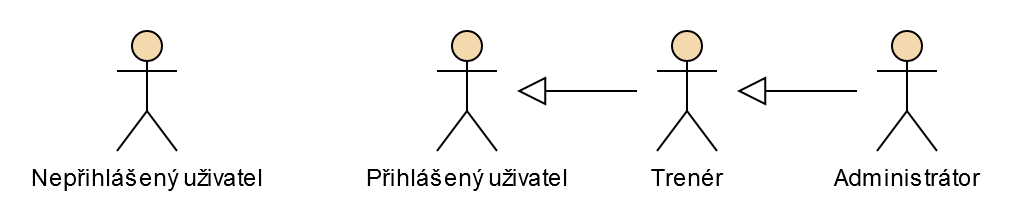
\includegraphics[width=\textwidth]{images/actors}
\end{figure}

\subsection{Případy užití}
\begin{enumerate}[label=\textcolor{decoration}{\textbf{UC\arabic*}}, leftmargin=1cm, align=left, labelwidth=8mm]

	\myItem{registrace}
	Před~prvním prací se systémem se musí člen klubu zaregistrovat. 
	\begin{enumerateNumbers}
		\item Nepřihlášený uživatel klikne na~položku \emph{Registrace} v~hlavní nabídce.
		\item Pro~úspěšné dokončení registrace musí vyplnit svou e-mailou adresu, heslo, jméno a~příjmení a~kliknout na~tlačítko \emph{Registrovat}.
		\item Registraci musí následně schválit některý z~administrátorů a~poté se již nepřihlášený uživatel může pomocí zadané e-mailové adresy a~hesla přihlásit do~systému.
	\end{enumerateNumbers}

	\myItem{přihlášení a~odhlášení z~aplikace}
	Nepřihlášený uživatel bude při~pokusu o~přístup do~systému vyzván k~přihlášení.
	\begin{enumerateNumbers}
		\item Nepřihlášený uživatel zadá svou e-mailovou adresu a~heslo a~klikne na~tlačítko \emph{Přihlásit}.
		\item Uživatel bude přesměrován na~hlavní stránku aplikace nebo~na~stránku, na~kterou se snažil před~přihlášením přistoupit.
		\item Přihlášený uživatel má naopak možnost se ze~systému odhlásit kliknutím na~položku \emph{Odhlásit} v~hlavní nabídce.
	\end{enumerateNumbers}	

	\myItem{zobrazení seznamu událostí\label{uc:listevents}}
	Tento případ užití popisuje proces zobrazení seznamu událostí evidovaných v~systému.
	\begin{enumerateNumbers}
		\item Přihlášený uživatel klikne na~položku \emph{Události} v~hlavní nabídce.
		\item Ve~výchozím nastavení se zobrazují všechny nadcházející události, avšak upravením nastavení v~horní části stránky lze zobrazit i~minulé události nebo~provést filtraci na~základě typu události, případně na~základě typu závodu.
		\item Na~jedné stránce se vždy zobrazuje maximální 25~událostí, další události je možné zobrazit přejitím na~další (předchozí) stránku.
	\end{enumerateNumbers}

	\myItem{zobrazení detailních informací o~události\label{uc:eventdetail}}
	Tento případ užití popisuje proces zobrazení detailních informací o~konkrétní události.
	\begin{enumerateNumbers}
		\item Přihlášený uživatel se může prokliknout na~stránku s~informacemi o~události z(e):
		\begin{enumerate}[label=\textcolor{decoration}{\textbf{\alph*.}}]
			\item seznamu událostí (viz~\ref{uc:listevents}).
			\item hlavní stránky, kde se zobrazuje 5~událostí, u~kterých nejdříve končí uzávěrka přihlášek, a~5~nejbližších událostí, na~které je uživatel přihlášený.
		\end{enumerate}
		\item Na~této stránce jsou následně zobrazeny všechny informace o~události, které se v~systému evidují (seznam evidovaných informací viz~\ref{f:events}).
	\end{enumerateNumbers}

	\myItem{přihlášení na~událost}
	Přihlášení na~událost je možné provést pouze pokud neproběhla uzávěrka přihlášek a~pokud již není daný uživatel na~danou událost přihlášený.
	\begin{enumerateNumbers}
		\item Přihlášený uživatel přejde na~stránku s~detailními informacemi o~události (viz~\ref{uc:eventdetail}).
		\item Uživatel vybere jednu z~nabízených kategorií a~volitelně sdělí, zda má možnost jet vlastním autem a~svézt s~sebou i~další členy klubu.
		\item Účast na~události potvrdí kliknutím na~tlačítko \emph{Přihlásit}.
	\end{enumerateNumbers}

	\myItem{odhlášení z~události}
	Odhlášení z~události je možné provést pouze pokud neproběhla uzávěrka přihlášek a~pokud je daný uživatel na~danou událost přihlášený.
	\begin{enumerateNumbers}
		\item Přihlášený uživatel přejde na~stránku s~detailními informacemi o~události (viz~\ref{uc:eventdetail}).
		\item Účast na~události uživatel zruší kliknutím na~tlačítko \emph{Odhlásit}.
	\end{enumerateNumbers}

	\myItem{napsání komentáře}
	Tento případ užití popisuje přidání komentáře ke~konkrétní události.
	\begin{enumerateNumbers}
		\item Přihlášený uživatel přejde na~stránku s~detailními informacemi o~události (viz~\ref{uc:eventdetail}).
		\item Po~napsání komentáře do~příslušného textového pole klikne na~tlačítko \emph{Odeslat}.
	\end{enumerateNumbers}

	\myItem{úprava osobních údajů a~preferencí}
	\myItem{přidání události}
	\myItem{úprava události}
	\myItem{synchronizace přihlášek}
	\myItem{vytvoření oznámení}
	\myItem{úprava uživatele}
\end{enumerate}

\subsection{Pokrytí funkčních požadavků případy užití}
V~tabulce \ref{table:use-cases} je zachyceno pokrytí funkčních požadavků v~jednotlivých případech užití. Symbol~\Checkmark říká, že příslušný funkční požadavek je součástí daného případu užití.

\begin{table}[h]
	\centering
	\caption{\label{table:use-cases}Mapování funkčních požadavků na případy užití}
	\begin{tabularx}{0.95\textwidth}{|C||C|C|C|C|C|C|C|}
		\hline
			 & F1 & F2 & F3 & F4 & F5 & F6 & F7 				\\ \hline\hline
		UC1  & \Checkmark &    &    &    &    &    &    		\\ \hline
		UC2  & \Checkmark &    &    &    &    &    &    		\\ \hline
		UC3  &    & \Checkmark &    &    &    &    &    		\\ \hline
		UC4  &    & \Checkmark &    &    &    &    &    		\\ \hline
		UC5  &    &    & \Checkmark &    &    &    &    		\\ \hline
		UC6  &    &    & \Checkmark &    &    &    &    		\\ \hline
		UC7  &    &    &    &    &    &    & \Checkmark 		\\ \hline
		UC8  & \Checkmark &    &    &    & \Checkmark &    &	\\ \hline
		UC9  &    & \Checkmark &    &    & \Checkmark &    &	\\ \hline
		UC10 &    & \Checkmark &    &    &    &    &    		\\ \hline
		UC11 &    &    &    & \Checkmark &    &    &    		\\ \hline
		UC12 &    &    &    &    &    & \Checkmark &    		\\ \hline
		UC13 & \Checkmark &    &    &    &    &    &    		\\ \hline
	\end{tabularx}
\end{table}
